\documentclass[12pt,a4paper]{article}
\usepackage[utf8]{inputenc}
\usepackage[T1]{fontenc}
\usepackage{amsmath,amssymb,amsfonts}
\usepackage{geometry}
\usepackage{graphicx}
\usepackage{listings}
\usepackage{xcolor}
\usepackage{hyperref}
\usepackage{booktabs}
\usepackage{array}
\usepackage{tikz}
\usetikzlibrary{arrows.meta,shapes,positioning}

\geometry{margin=2.5cm}

\lstset{
  basicstyle=\ttfamily\small,
  keywordstyle=\color{blue}\bfseries,
  commentstyle=\color{gray},
  stringstyle=\color{red},
  breaklines=true,
  frame=single,
  backgroundcolor=\color{gray!5}
}

\title{\textbf{Report 1: Inter-Process Communication Architecture}\\
\large uORB Messaging, XRCE-DDS Bridge, AutosoaringControl, and AutosoaringStatus\\[0.5em]
\normalsize PX4 Autosoaring Implementation --- Defence Technical Report}
\author{Radhouene --- Fixed-Wing Autosoaring Project}
\date{April 2026}

\begin{document}
\maketitle
\tableofcontents
\newpage

%=============================================================================
\section{Introduction}
%=============================================================================

This report describes the inter-process communication (IPC) infrastructure
used to command the autosoaring system from a ROS\,2 companion computer to
the PX4 flight management unit (FMU). It covers:

\begin{itemize}
  \item the uORB publish-subscribe middleware;
  \item the XRCE-DDS bridge that connects ROS\,2 to uORB;
  \item the original messaging approach (boolean flags);
  \item the redesigned \texttt{AutosoaringControl} message using a single
        enumerated mode integer;
  \item the \texttt{AutosoaringStatus} message published by the FMU so the
        companion can observe \texttt{soar:off} (including the 5\,s DDS inhibit
        deadline) and staleness-forced shutdowns.
\end{itemize}

%=============================================================================
\section{Original System: uORB and the Absence of Soaring IPC}
%=============================================================================

\subsection{uORB Publish-Subscribe Middleware}

PX4 uses \emph{uORB} (micro Object Request Broker) as its internal IPC
bus. It is a strongly-typed, zero-copy, publish-subscribe system running
entirely inside the NuttX RTOS process space. Each \emph{topic} is defined
by a \texttt{.msg} file and compiled into a C struct. Publishers call
\texttt{orb\_publish()}, subscribers call \texttt{orb\_subscribe()} and
\texttt{orb\_copy()}.

Key properties:
\begin{itemize}
  \item \textbf{Single writer, multiple readers}: uORB supports one active
        publisher per topic instance. Multiple modules may subscribe.
  \item \textbf{Non-blocking}: \texttt{orb\_check()} tests for new data
        without blocking. Blocking waits use \texttt{px4\_poll()}.
  \item \textbf{Fixed-size structs}: every message has a 64-bit
        \texttt{timestamp} field plus typed payload fields.
\end{itemize}

\subsection{XRCE-DDS Bridge}

The \texttt{uxrce\_dds\_client} module implements the
\emph{DDS-XRCE} (eXtremely Resource Constrained Environments) protocol,
bridging uORB topics to a ROS\,2 DDS domain:

\begin{center}
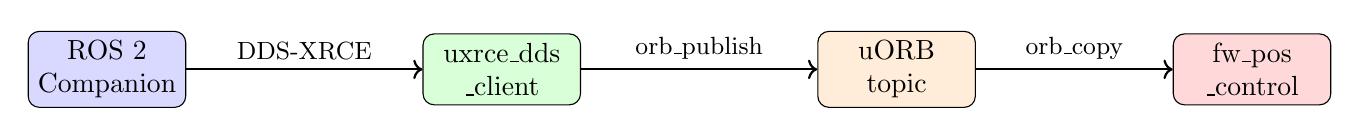
\begin{tikzpicture}[node distance=2.5cm, auto,
    box/.style={draw,rounded corners,minimum width=2.0cm,minimum height=0.8cm,align=center}]
  \node[box,fill=blue!15] (ros) {ROS 2\\Companion};
  \node[box,fill=green!15,right=3cm of ros] (dds) {uxrce\_dds\\\_client};
  \node[box,fill=orange!15,right=3cm of dds] (uorb) {uORB\\topic};
  \node[box,fill=red!15,right=2.5cm of uorb] (mod) {fw\_pos\\\_control};
  \draw[->,thick] (ros) -- node[above]{\small DDS-XRCE } (dds);
  \draw[->,thick] (dds) -- node[above]{\small orb\_publish} (uorb);
  \draw[->,thick] (uorb) -- node[above]{\small orb\_copy} (mod);
\end{tikzpicture}
\end{center}

The bridge is configured in \texttt{dds\_topics.yaml}. Topics listed under
\texttt{subscriptions} flow from ROS\,2 \emph{into} the FMU
(\texttt{/fmu/in/}); topics under \texttt{publications} flow out.

\subsection{Original dds\_topics.yaml (no soaring)}

In the original \emph{Music} codebase, \texttt{dds\_topics.yaml} contained
no entry for autosoaring. The companion computer had no standardised channel
to command soaring behaviour; workarounds relied on MAVLink parameter
setting or ad-hoc MAVLink commands.

%=============================================================================
\section{Modified System: AutosoaringControl Message Design}
%=============================================================================

\subsection{Design Rationale: From Two Booleans to One Integer}

The first prototype used two boolean fields:
\texttt{glide\_mode\_enabled} and \texttt{thermal\_mode\_enabled}.
This creates $2^2 = 4$ possible combinations, two of which are ambiguous:

\begin{center}
\begin{tabular}{ccp{6cm}}
\toprule
\texttt{glide} & \texttt{thermal} & Interpretation \\
\midrule
\texttt{false} & \texttt{false} & powered flight \\
\texttt{true}  & \texttt{false} & glide mode \\
\texttt{false} & \texttt{true}  & thermal mode \\
\texttt{true}  & \texttt{true}  & \textbf{ambiguous --- both asserted} \\
\bottomrule
\end{tabular}
\end{center}

Furthermore, a separate PX4 parameter \texttt{FW\_GLIDE\_MODE} (integer
0 or 1) controlled whether the glide airspeed used a fixed value or the
polar-optimal speed, creating a \emph{hidden third dimension} invisible in
the uORB message.

The redesign encodes all five states in a single \texttt{uint8
soaring\_mode} field:

\begin{center}
\begin{tabular}{clll}
\toprule
Value & Constant & TECS behaviour & Navigator state \\
\midrule
0 & \texttt{SOARING\_OFF}            & powered        & unchanged \\
1 & \texttt{SOARING\_GLIDE\_FIXED}   & gliding, fixed EAS & AUTO\_MISSION \\
2 & \texttt{SOARING\_GLIDE\_POLAR}   & gliding, polar EAS & AUTO\_MISSION \\
3 & \texttt{SOARING\_THERMAL\_LOITER}& gliding        & AUTO\_LOITER (navigator-guided) \\
4 & \texttt{SOARING\_THERMAL\_BANK}  & gliding        & AUTO\_LOITER (roll override) \\
\bottomrule
\end{tabular}
\end{center}

\subsection{Complete AutosoaringControl Message}

\begin{lstlisting}[language=,caption={AutosoaringControl.msg (new)}]
uint64  timestamp               # microseconds since boot

uint8   soaring_mode            # see constants below
uint8 SOARING_OFF             = 0
uint8 SOARING_GLIDE_FIXED     = 1
uint8 SOARING_GLIDE_POLAR     = 2
uint8 SOARING_THERMAL_LOITER  = 3
uint8 SOARING_THERMAL_BANK    = 4

# Loiter geometry (mode 3 only)
float32 loiter_radius_m         # [m]; NaN => bank-derived minimum
float32 loiter_lat              # [deg]; NaN/0 => current position
float32 loiter_lon              # [deg]; NaN/0 => current position

# Optimisation commands (NaN => PX4 parameter default)
float32 airspeed_cmd            # [m/s EAS]  mode 1 only
float32 bank_angle_cmd          # [deg]       modes 3 and 4
bool    loiter_clockwise        # true=CW, false=CCW

# Metadata
uint8   soaring_phase
uint8 SOARING_PHASE_CRUISE    = 0
uint8 SOARING_PHASE_GLIDING   = 1
uint8 SOARING_PHASE_SEARCHING = 2
uint8 SOARING_PHASE_CENTERING = 3
uint8 SOARING_PHASE_THERMAL   = 4
\end{lstlisting}

\subsection{Field Usage Matrix}

\begin{center}
\begin{tabular}{lccccc}
\toprule
Field & Mode 0 & Mode 1 & Mode 2 & Mode 3 & Mode 4 \\
\midrule
\texttt{airspeed\_cmd}    & --   & \checkmark & --         & --  & -- \\
\texttt{loiter\_radius\_m}& --   & --         & --         & \checkmark & -- \\
\texttt{loiter\_lat/lon} & --   & --         & --         & \checkmark & -- \\
\texttt{bank\_angle\_cmd} & --   & --         & --         & \checkmark & \checkmark \\
\texttt{loiter\_clockwise}& --   & --         & --         & \checkmark & \checkmark \\
\texttt{soaring\_phase}   & \checkmark & \checkmark & \checkmark & \checkmark & \checkmark \\
\bottomrule
\end{tabular}
\end{center}

\subsection{Registration in dds\_topics.yaml}

\textbf{Companion $\rightarrow$ FMU} (subscription side of the client):

\begin{lstlisting}[language=,caption={Addition to dds\_topics.yaml (subscriptions)}]
subscriptions:
  ...
  - topic: /fmu/in/autosoaring_control
    type: px4_msgs::msg::AutosoaringControl
\end{lstlisting}

This enables the bridge to forward ROS\,2 messages published on
\texttt{/fmu/in/autosoaring\_control} into the FMU uORB bus.

\textbf{FMU $\rightarrow$ companion} (publication side):

\begin{lstlisting}[language=,caption={Addition to dds\_topics.yaml (publications)}]
publications:
  ...
  - topic: /fmu/out/autosoaring_status
    type: px4_msgs::msg::AutosoaringStatus
\end{lstlisting}

The \texttt{fw\_pos\_control} module publishes \texttt{autosoaring\_status} on
uORB; the bridge exposes it to ROS\,2 as \texttt{/fmu/out/autosoaring\_status}.

\subsection{AutosoaringStatus message (FMU $\rightarrow$ companion)}

\begin{lstlisting}[language=,caption={AutosoaringStatus.msg}]
uint64 timestamp
uint8 source
uint8 SOURCE_CLI_SOARING_OFF     = 0   # operator soar:off (CUSTOM_0, mode 0)
uint8 SOURCE_STALENESS_WATCHDOG  = 1   # companion silent >2 s
uint8 SOURCE_PERIODIC            = 2   # 2 Hz heartbeat while soaring active
uint8 soaring_mode_effective     # same encoding as AutosoaringControl.soaring_mode
uint64 dds_inhibit_until_us      # absolute HRT time [us]; 0 = no DDS inhibit
uint8 fmu_soaring_phase
uint8 SOARING_PHASE_CRUISE       = 0   # powered cruise (soaring OFF)
uint8 SOARING_PHASE_GLIDING      = 1   # engine-off glide along mission
uint8 SOARING_PHASE_SEARCHING    = 2   # thermal active, loiter centre not yet set
uint8 SOARING_PHASE_THERMAL      = 3   # thermal loiter, centre established
\end{lstlisting}

The field \texttt{dds\_inhibit\_until\_us} is set when the operator issues
\texttt{soar:off}: the FMU ignores DDS attempts to re-enable soaring until that
timestamp (5\,s after the command). The companion can subscribe to this topic
and align its publishes (e.g.\ send \texttt{SOARING\_OFF} or stop asserting
soaring on) before the inhibit window ends. While the inhibit is active,
\texttt{fw\_pos\_control} republishes status at 1\,Hz for packet-loss robustness.

The field \texttt{fmu\_soaring\_phase} reflects what the FMU is \emph{actually
executing} each cycle, regardless of what the companion requested. This gives
the companion an independent confirmation of the real flight phase, and the
value is recorded in ULog via uORB so the phase history is available
post-flight. During active soaring, a \texttt{SOURCE\_PERIODIC} message is
emitted at 2\,Hz so the companion always has a fresh phase estimate.

\subsection{Staleness Watchdog}

A companion-silence detector is implemented in
\texttt{FixedwingPositionControl::Run()}:

\begin{equation}
  \Delta t_{\text{silence}} = t_{\text{now}} - t_{\text{last\_recv}}
\end{equation}

If $\Delta t_{\text{silence}} > 2\,\text{s}$ and
\texttt{soaring\_mode} $\neq 0$, the FMU autonomously sets
\texttt{soaring\_mode} $\leftarrow 0$ (off) and disables gliding in TECS.
It also publishes \texttt{AutosoaringStatus} with
\texttt{SOURCE\_STALENESS\_WATCHDOG} and \texttt{dds\_inhibit\_until\_us = 0}.
This prevents the aircraft from remaining in engine-off glide indefinitely
if the companion crashes or the DDS link is lost.

\subsection{CLI Override Path}

For ground testing without a companion, the Commander module accepts CLI
commands:

\begin{lstlisting}[language=bash]
commander mode soar:glide    # mode 1
commander mode soar:polar    # mode 2
commander mode soar:thermal  # mode 3
commander mode soar:bank     # mode 4
commander mode soar:off      # mode 0
\end{lstlisting}

Each command sends \texttt{VEHICLE\_CMD\_CUSTOM\_0} with \texttt{param1}
equal to the soaring mode integer.

When \textbf{enabling} soaring (\texttt{param1} $\neq 0$), the CLI path sets
\texttt{\_soaring\_local\_override = true}, which bypasses:
\begin{itemize}
  \item staleness watchdog (no companion expected when CLI is in control);
  \item any active DDS inhibit (the inhibit timer is cleared to allow DDS
        cooperation immediately after the CLI command).
\end{itemize}

\noindent
The altitude floor (\texttt{FW\_ALT\_MIN}) is \textbf{not} bypassed, even in
CLI mode. If the aircraft descends below \texttt{FW\_ALT\_MIN} while soaring
is active, the FMU:
\begin{enumerate}
  \item sets \texttt{\_soaring\_forbidden\_latched = true} and clears
        \texttt{\_soaring\_local\_override};
  \item disables TECS gliding mode (throttle is restored);
  \item publishes \texttt{VEHICLE\_CMD\_DO\_SET\_MODE $\to$ AUTO\_MISSION} so
        the navigator resumes the pre-soaring flight plan.
\end{enumerate}
\noindent
This design ensures that a pilot testing via CLI at low altitude does not
inadvertently fly the aircraft into the ground. The operator must re-issue
\texttt{soar:glide} or \texttt{soar:polar} once sufficient altitude has been
recovered.

When \textbf{disabling} soaring (\texttt{soar:off}, \texttt{param1} $= 0$),
\texttt{\_soaring\_local\_override} is cleared, a 5\,s DDS inhibit is started,
and the FMU publishes \texttt{AutosoaringStatus} with
\texttt{SOURCE\_CLI\_SOARING\_OFF} and \texttt{dds\_inhibit\_until\_us} set to
the absolute deadline (see above).

%=============================================================================
\section{Summary of Changes}
%=============================================================================

\begin{center}
\begin{tabular}{p{4cm}p{5cm}p{5cm}}
\toprule
Aspect & Original & Modified \\
\midrule
Mode encoding & Two separate booleans + hidden parameter & Single \texttt{uint8 soaring\_mode} \\
Polar selection & PX4 parameter \texttt{FW\_GLIDE\_MODE} & Encoded in \texttt{soaring\_mode} = 2 \\
DDS registration & Not present & \texttt{/fmu/in/autosoaring\_control} in \texttt{dds\_topics.yaml} \\
FMU status to companion & Not present & \texttt{/fmu/out/autosoaring\_status} + \texttt{AutosoaringStatus.msg} \\
Turn direction & Not supported & \texttt{loiter\_clockwise} bool \\
Staleness guard & Not present & 2-second watchdog in Run() (+ status publish) \\
CLI commands & \texttt{soar:glide}, \texttt{soar:thermal}, \texttt{soar:off} & + \texttt{soar:polar}, \texttt{soar:bank} \\
\bottomrule
\end{tabular}
\end{center}

\end{document}
